% Journal Article
% LaTeX Template
% Version 2.0 (February 7, 2023)
%
% This template originates from:
% https://www.LaTeXTemplates.com
%
% Author:
% Vel (vel@latextemplates.com)
%
% License:
% CC BY-NC-SA 4.0 (https://creativecommons.org/licenses/by-nc-sa/4.0/)
%
% NOTE: The bibliography needs to be compiled using the biber engine.
%
%%%%%%%%%%%%%%%%%%%%%%%%%%%%%%%%%%%%%%%%%

%----------------------------------------------------------------------------------------
%	PACKAGES AND OTHER DOCUMENT CONFIGURATIONS
%----------------------------------------------------------------------------------------

\documentclass[
	letterpaper, % Paper size, use either a4paper or letterpaper
	12pt, % Default font size, can also use 11pt or 12pt, although this is not recommended
	unnumberedsections, % Comment to enable section numbering
	twoside, % Two side traditional mode where headers and footers change between odd and even pages, comment this option to make them fixed
]{LTJournalArticle}

\addbibresource{bibliography.bib} % BibLaTeX bibliography file

\runninghead{Manipulative Language Detection in LLM-Crafted Phishing Attacks} % A shortened article title to appear in the running head, leave this command empty for no running head

\footertext{\textit{Final Project} (MICS/DATSCI 266, Summer 2025)} % Text to appear in the footer, leave this command empty for no footer text

\setcounter{page}{1} % The page number of the first page, set this to a higher number if the article is to be part of an issue or larger work

%----------------------------------------------------------------------------------------
%	TITLE SECTION
%----------------------------------------------------------------------------------------

\usepackage[title,toc,titletoc]{appendix}
\usepackage{titlesec}
\usepackage{lscape}
\usepackage{fontawesome}


\title{Manipulative Language Detection in LLM-Crafted
Phishing Attacks
}  % Article title, use manual lines breaks (\\) to beautify the layout}

% Authors are listed in a comma-separated list with superscript numbers indicating affiliations
% \thanks{} is used for any text that should be placed in a footnote on the first page, such as the corresponding author's email, journal acceptance dates, a copyright/license notice, keywords, etc
\author{
	Karl-Johan Westhoff \\
	email: \href{mailto:kjwesthoff@berkeley.edu}{kjwesthoff@berkeley.edu} \\
    Neha Dhage \\
	email: \href{mailto:neha_dhage@ischool.berkeley.edu}{neha\_dhage@ischool.berkeley.edu}
}


% Affiliations are output in the \date{} command
\date{UC Berkeley School of Information \\
MIDS Course 266 Summer 2025 Section 2 (Natalie Ahn) \\
}

% % Full-width abstract
% \renewcommand{\maketitlehookd}{%
% 	\begin{abstract}
% 		\noindent Lorem ipsum dolor sit amet,rta porttitor.
% 	\end{abstract}
% }

%----------------------------------------------------------------------------------------
\setcounter{tocdepth}{5}
\setcounter{secnumdepth}{5}
\usepackage[title]{appendix}

\begin{document}
\maketitle % Output the title section
%----------------------------------------------------------------------------------------
%	ARTICLE CONTENTS
%----------------------------------------------------------------------------------------
\section{Introduction}
The human factor remains central in cyber attacks. The 2024 Verizon DBIR report \cite{verizon2024dbir} notes that 68\% of breaches involve the human element, with phishing as a key contributor. With LLM tools, bad actors can now craft highly convincing phishing messages that evade traditional detection.
This project investigates whether NLP models can detect manipulative language—specifically, text designed to influence actions not in the reader's best interest.

Machine learning (ML) models like Naive Bayes and basic neural networks are widely used to filter email traffic for spam (which is an abundant problem). However, they are often limited to detecting specific words or obvious patterns. Newer approaches combine lightweight ML filtering with resource-heavy NLP methods for cases that are not clearly categorized by simpler filtering. Since phishing often exploits human psychology through language, this study focuses on detecting manipulative language and whether such detection may improve defenses against phishing. Although the focus is on cybersecurity, manipulative language also appears in areas such as coercive or abusive communication, highlighting its broader relevance. Our approach first models manipulation using the “Mental Manip” dataset, then explores its potential for phishing detection.

\section{Literature}
Salloum et al. \cite{SALLOUM202119} provide an overview of current ML and NLP methods used for phishing detection, which forms the foundational context for this project.
Suhaima et al. \cite{ImprovedPhishing} trained models like BERT on spam data, whereas our focus will be on specifically detecting manipulative language.
Wang et al. \cite{MentalManip} created a data set aiming at dialogue manipulation, which will serve as our primary training set.
Al-Subaiey et al. have compiled a large corpus of emails in \cite{PhishingEmailDataset} from various datasets, under phishing-specific email body texts; this will be used for attempts to detect phishing texts.

\section{Datasets}
Labeled data sets focused on manipulation are rare. Most of the research has come from psychology, which provides insight into the techniques used for manipulation rather than bulk data suitable for AI model training. Most existing data sets suitable for NLP applications are concerned with hate speech and abusive language, which has been an important topic in relation to social media.

\section{The MentalManip Dataset}
Wang et al. \cite{MentalManip} introduced the "MentalManip" dataset, published on hugging face \cite{MentalManipDataset}. The data set is based on fictional dialogues from "The Cornell Movie Dialogs Corpus" \cite{CornellMovieCorpus} from which suitable manipulative dialogues were selected using BERT and GPT-4 models, from these, 4000 dialogues were manually selected to form the data set. The data is labeled with a detailed manipulation taxonomy in three dimensions; see Figure \ref{fig:Taxonomy}, adding applied technique and psychological vulnerability mechanism to the binary presence of whether the dialogue contains manipulation or not.
\begin{figure}[!htp] % Single column :figure	
	\centering
	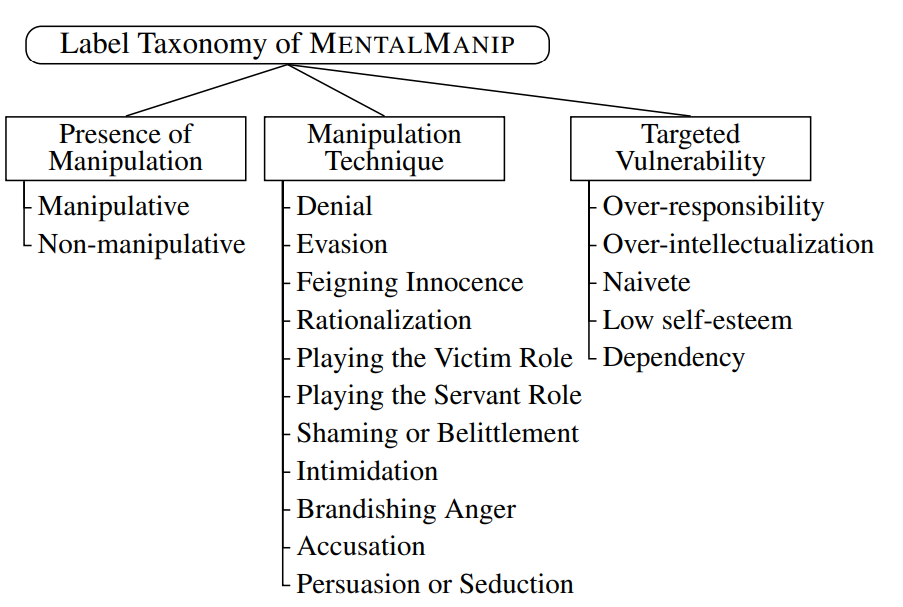
\includegraphics[width=0.5\textwidth]{Taxonomy.png}
	\caption{Taxonomy labels in the data set}
	\label{fig:Taxonomy}
\end{figure}

The data set was manually labeled using a multi-phase human annotation process, adapting the taxonomy (Figure \ref{fig:Taxonomy}) to the dialogue context three times by different people annotating. This gave two versions of the data set, one where the majority two out of three constitutes the result ("$MentalManip_{maj}$") and one where all three annotators have consensus and reach the same results ("$MentalManip_{con}$"). The $MentalManip_{maj}$ data set is larger (4000 rows) and more suitable for training a model capturing more instances of manipulation, the $MentalManip_{con}$ data set is smaller (2920 rows) and more precise and better suited for fine tuning. For this project we used the $MentalManip_{maj}$ data.

\subsection{Data Exploration}\label{sec:DataExploration}
In some cases these data fields are not complete in the data set requiring some degree of feature manipulation, This is addressed in section \ref{sec:FeatureEngineering} below.

\subsection{Dialogues}
The 4000 dialogues in the data set are between two persons exchanging sentences. By far the majority of dialogues consist of two exchanges, one by each person (there are only three cases with three exchanges). Word count statistics are shown in Figure \ref{fig:DialogueWordCount}, most dialogues consist of up to 50 words per person, and the number of words uttered by each person is fairly balanced, with person 2 saying slightly more words than person 1 in the up to 50 word majority case. Figure \ref{fig:DialogueEmbedding} shows the distribution of token counts for the dialogues in the data set, tokenized using BERT-base as reference. Only a minor number of dialogues exceed the BERT-base embedding size of 512 tokens.


\begin{figure}[!htp] % Single column :figure	
	\centering
	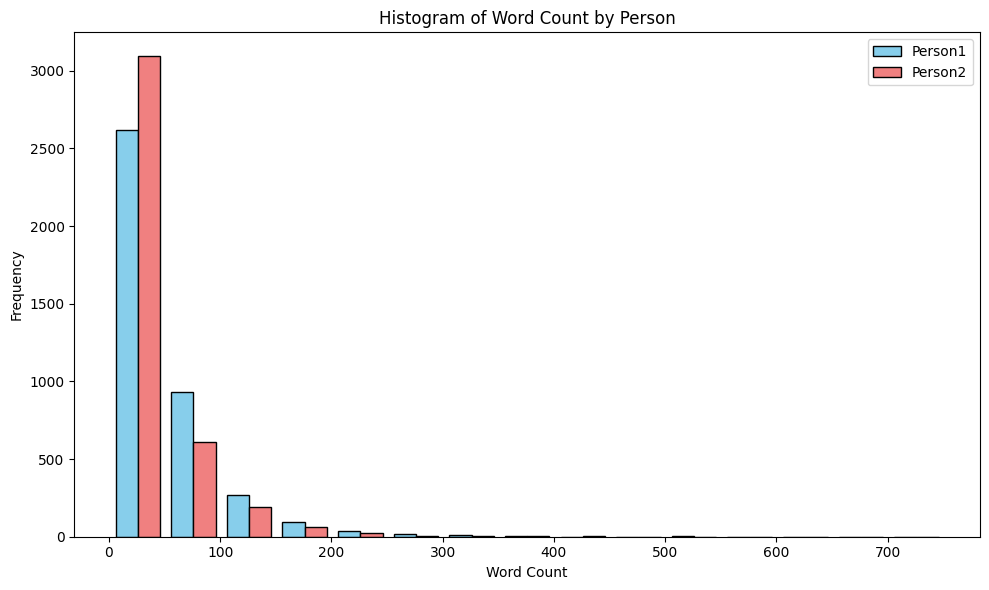
\includegraphics[width=0.5\textwidth]{DialogueWordCountStats.png}
	\caption{Word count statistics for the dialogues in the $MentalManip_{maj}$ data set, words uttered by each person}
	\label{fig:DialogueWordCount}
\end{figure}

\begin{figure}[!htp] % Single column :figure	
	\centering
	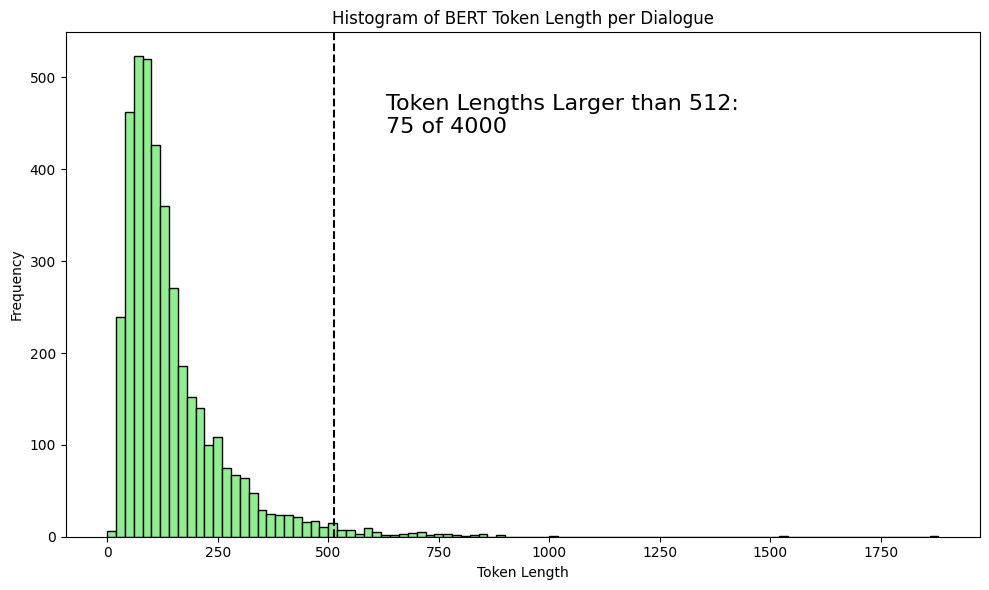
\includegraphics[width=0.5\textwidth]{DialogueEmbeddingStats.png}
	\caption{Statistics for the dialogue in the $MentalManip_{maj}$ data set, tokenized using BERT-base}
	\label{fig:DialogueEmbedding}
\end{figure}


\subsection{Labels}

\subsubsection{Manipulation Label}
The data set is not split equally between manipulation and non-manipulation, Figure \ref{fig:ManipulationRatio} shows the distribution with 2.4 times more manipulation rows than non-manipulation (discussed in section \ref{sec:FeatureEngineering}).

\begin{figure}[!htp] % Single column :figure	
	\centering
	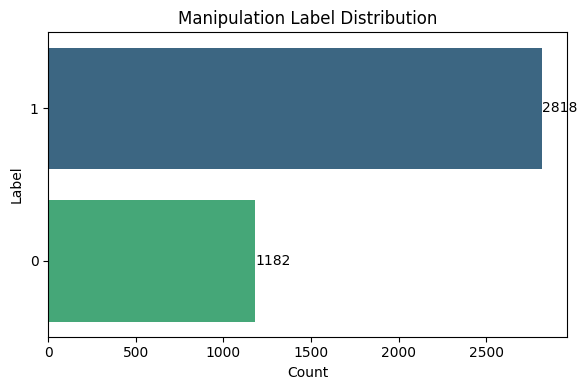
\includegraphics[width=0.5\textwidth]{ManipulationRatio.png}
	\caption{Ratio of manipulation to non-manipulation in the $MentalManip_{maj}$ Dataset}
	\label{fig:ManipulationRatio}
\end{figure}

\subsubsection{'Technique' and 'Vulnerability' Labels}
Some of the labels are missing for some of the rows with manipulation present\footnote{The labels should not be populated for non-manipulation rows}, Figure \ref{fig:MissingLabels} shows a total of 664\footnote{110 missing technique and 554 also missing vulnerability} missing labels for 'technique', we regard the technique labels as most relevant for phishing, especially the 'Persuasion or Seduction' label.
\begin{figure}[!htp] % Single column :figure	
	\centering
	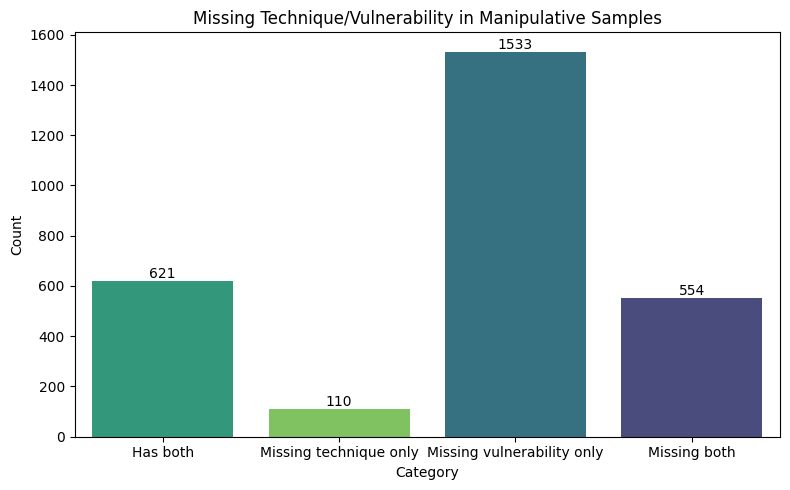
\includegraphics[width=0.5\textwidth]{MisingLabels.png}
	\caption{Incomplete labeling of the MentalManip Dataset}
	\label{fig:MissingLabels}
\end{figure}


\begin{figure}[!htp] % Single column :figure	
	\centering
	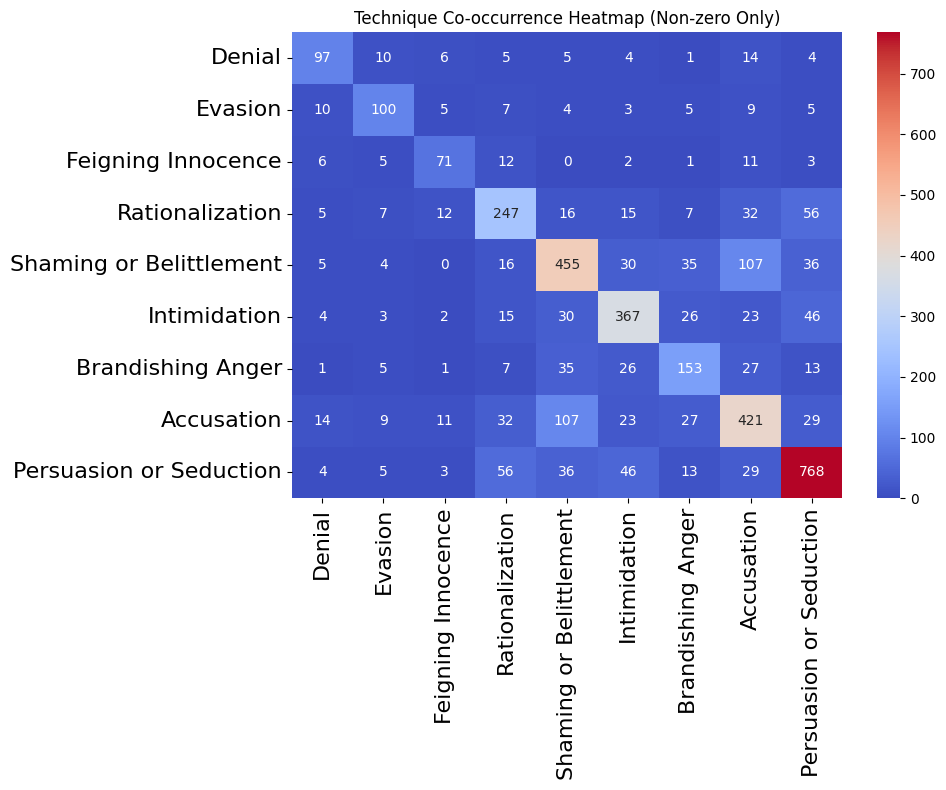
\includegraphics[width=0.5\textwidth]{TechniqueCoOcurrence.png}
	\caption{Distribution and Co-ocurrence of technique labels}
	\label{fig:TechCoOcurrence}
\end{figure}

Further data exploration can be found in appendix \ref{appendix:DataExploration}




\section{Baselines}
With the relatively short embeddings (see Figure \ref{fig:DialogueEmbedding}), the more basic versions of BERT have sufficient capacity to handle the data. The MentalManip article \cite{MentalManip} also uses some decoder only models by 'zero' and 'few-shot' prompting the model with random example from the data set. This seems to perform better for overall binary classification, but only a little, and the LLM's have a tendency to pick up on toxicity and hate-speech and identify these as manipulation.
Considering the label inconsistencies for 'technique' and 'vulnerability' in the data set, we will focus on the binary classification of manipulation for choosing a baseline model for further experimentation.


\subsection{Binary with BERT and Buddies}
Models looking at the 'manipulative' labels are trained on the $MentalManip_{maj}$ data set. The models were run with similar parameters, and the Accuracy at epoch before significant over fitting\footnote{Significant over fitting defined as: training loss / evaluation loss < 0.6} recorded. Following models were investigated:
\begin{itemize}
	\item BERT-base \cite{BERT-base}
	\item RoBERTa \cite{RoBERTa}
	\item DistilBERT \cite{DistilBERT}
	\item ModernBERT \cite{ModernBERT}
	\item DeBERTaV3 \cite{DeBERTaV3}
\end{itemize}
Furthermore some "emotionally wiser" BERT derivatives exist which are pre-trained for emotion detection:
\begin{itemize}
	\item BERTweet \cite{BERTweet}
	\item EmotionBERT \cite{EmotionBERT}
\end{itemize}

\subsection{Baseline Results and Discussion}\label{sec:BaselineResults}
Results with losses and accuracy are shown in Table \ref{tab:BaseModelPerformance}. The models were run until significant over-fitting occurred. In general the models over-fit after a few epochs which is to be expected with a model that is extended from pre-trained. The Accuracy results are around 0.70-0.72 with little variation. Models can be found in Appendix \ref{appendix:BaseCaseModels}

\subsubsection{ModernBERT} The model does not perform better, this was expected as the embedding lengths are short (see Figure \ref{fig:DialogueEmbedding}) and not leveraging the benefits of ModernBERTs larger capacity.

\subsubsection{Emotionally intelligent BERT}
BERTweet performs on par with BERT-base, the model is primarily trained for "Part-of-speech tagging", "Named-entity recognition" and "text classification" \cite{BERTweet} herunder including emjojis etc. i.e. The model is not per-se expected to be better at manipulation detection, but we thought to give it a try. The EmotionBERT model was created for multi label classification of well known emotional phrases for media monitoring \cite{EmotionBERT}.

\subsubsection{Advanced BERT}
We also tried some more advanced BERT derivatives (DestilBERT and deBERTa\_v3\_small), however these models did not perform better than RoBERTa, and they required more compute resources to train. DeBERTa uses more advanced training loss, pre-training more advanced encoding etc.\cite{DeBERTaV3}, however only the smallest version of deBERTa was possible to train with the hardware available. These models are optimized to deliver faster inference, but the extra cost in training resources make them less feasible for this project.
\subsubsection{RoBERTa}
The best performing model reported in Table \ref{tab:BaseModelPerformance} was RoBERTa, which seems to perform slightly better than BERT-base, however with multiple tries the performance was not consistent, sometimes BERT performed better, however RoBERTa seemed more stable giving consistent results above 0.72 and performing more Epochs before over-fitting.


\begin{table}[h!]
	\small
	\begin{tabular}{|p{2.2cm}|p{0.9cm}|p{1cm}|p{1cm}|p{1cm}|}
		\hline
		\textbf{Model} & \textbf{Epoch} & \textbf{Loss T/V} & \textbf{Acc Epoch} & \textbf{Acc Final} \\
		\hline
		BERT           & 2              & 0.97              & 0.726              & 0.70               \\
		roBERTa        & 4              & 1.03              & 0.728              & 0.73               \\
		deBERTa\_v3    & 3              & 0.68              & 0.704              & 0.72               \\
		DistilBERT     & 2              & 0.75              & 0.709              & 0.72               \\
		ModernBERT     & 2              & 0.81              & 0.718              & 0.72               \\
		BERTweet       & 2              & 0.97              & 0.705              & 0.70               \\
		EmotionBERT    & 2              & 1.04              & 0.704              & 0.70               \\


		\hline
	\end{tabular}
	\caption{Base Model performance comparison across different transformer architectures for binary inference on the "manipulative" column: Epochs before significant over-fitting, Training loss / Validation loss (to measure  overfitting) and accuracy at epoch and final classification }
	\label{tab:BaseModelPerformance}
\end{table}

\section{Fine Tuning}
Based on the results in section \ref{sec:BaselineResults}, we decided to fine tune the RoBERTa model with the $MentalManip_{maj}$ data set to see if we can get better results for the manipulation detection task. The MentalManip article\cite{MentalManip} achieved an accuracy of 0.78 which in itself is not impressive.

\subsection{LoRA/PEFT}
\subsection{Hyper parameters}






\section{Feature Engineering}\label{sec:FeatureEngineering}


\begin{itemize}
	\item Address the ratio (e.g. use only the persuasion or seduction labels)
	\item Manipulate the labels - maybe merge the best technique and vulnerability mechanism that fits phishing
	\item Remove rows with missing text data
	\item etc..
\end{itemize}

We address the missing labels (see Figure \ref{fig:MissingLabels}) by either removing the rows with missing labels, or by imputing the missing values with an 'Other' category for the experiments with multi-label inference.

\section{Experiments}
We will build an inference model that can detect manipulated emails based on a deep neural network with transformer architecture.

\section{Evaluation}
Our main interest is to investigate if the model can extend existing phishing detection systems by detecting manipulating language in the emails. We will to look at false negative results from previous models, to see if the detection of manipulative text captures emails that were previously missed.



\section{Conclusion}

The baseline investigations showed that applying the $MentalManip$ dataset to models optimized for emotional language detection does not automatically improve accuracy. Mental manipulation is less explored in literature than hate speech and abusive language, which are key concerns in social media, where sentiment analysis is both established and evolving in NLP.




%----------------------------------------------------------------------------------------
%	 REFERENCES
%----------------------------------------------------------------------------------------
\clearpage
\onecolumn
\printbibliography % Output the bibliography
%----------------------------------------------------------------------------------------

%----------------------------------------------------------------------------------------
%	 Appendices
%---------------------------------------------------------------------------------------


\begin{appendices}
	\onecolumn
	%
	\section{Data Exploration}\label{appendix:DataExploration}
	\url{https://github.com/KJWesthoff/266FinalProject/blob/main/Data-Exploration_MentalManip.ipynb}

	\section{BaseCaseModels}\label{appendix:BaseCaseModels}
	\url{https://github.com/KJWesthoff/266FinalProject/tree/main/BaseCaseModels}


\end{appendices}
%
\end{document}
